\documentclass[11pt]{article}
\usepackage{geometry}                
\geometry{letterpaper}
\usepackage[]{graphicx}
\usepackage{amssymb}
\usepackage{amsmath}
\usepackage{amsthm}
\usepackage{fancyhdr}
\usepackage{amsthm}
\usepackage[english]{babel}

\title{Exploiting Math.expm1(-0) in v8 TurboFan JIT Compiler}
\author{Ryan Torok, Sara McFearin, Michael Jarrett, Rachel Shi}
\date{December 7, 2019}
\begin{document}
\maketitle
\section{Introduction}
Browser bugs are difficult to find, but they appear to be prevalent across all four major browser
engines. In recent years most of the focus has been on bugs in the JavaScript Just-in-Time (JIT)
compilers. Improper optimization can often lead to a memory corruption exploit which allows the
attacker to take control of the victim's browser and begin executing aribtrary code on the victim's
machine, making browser bugs a popular target for cybercriminals who run botnets, ransomware scams,
and more. Although it is not uncommon for compilers to contain bugs in their large codebases,
browser JIT compilers are unique in the sense that they must deal with adversarially chosen code. In
a normal pre-compilation setting, if a compiler bug is found, programmers simply won't write code
that triggers the bug for sake of security. However, in browsers, the compiler runs on the user's
machine, and if a browser JIT compiler bug is found, attackers will intentionally ship code which
triggers the bug in order to take over the user's machine. 

With this in mind, it seems like we will be playing an infinite game of Whack-a-mole with browser
JavaScript engines, but new techniques have risen in recent years to make bug elimination faster,
most notably Fuzzing. Fuzzing is a technique which originated in image encoding protocols, where a
penetration tester will pass random binary inputs to the protocol attempting to cause a crash. With
some modifications based on knowledge of how browser JITs create a graph of a code segment,
penetration testers can write automated tools which generate random JavaScript code inputs which
look somewhat interesting. The most popular of these tools is called \textit{Fuzzily}, which has
already found a plethora of bugs in the JavaScript engines for all four major web browsers.

\section{The Bug}
\begin{figure}
	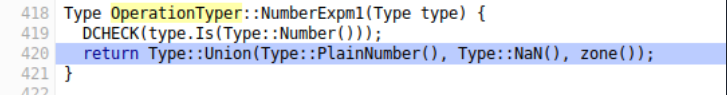
\includegraphics[width=\linewidth]{typer.png}
	\caption{The buggy return type declaration for Math.expm1() in operation-typer.cc}
  \label{fig:typer}
\end{figure}	
We will focus now on one of these bugs in particular. The TurboFan JIT compiler used by v8, the
JavaScript engine for the Chrome and Chromium web browsers, was exploited in 2018 using an edge case
with the function \texttt{Math.expm1()}, which computes $e^x -1$ for argument $x$.  Specifically, if
we evaluate \texttt{Math.expm1(-0)}, this should produce the value -0.  However, the TurboFan JIT
lists the return types for this function as a union of the \texttt{PlainNumber} type and NaN. This
union includes all values of a 64-bit floating point number, except -0. V8 defines this behavior
using a special table in typer.cc and operation-typer.cc. The code from the latter is shown in
Figure \ref{fig:typer}. The JIT uses this fine-grained type information to peform variable range
analysis that is used in array bounds check eliminations. For example, if TurboFan realizes a
boolean variable is used to index an array of length $\geq$ 2, then the native compiled code can
forgo ensuring the array index is in range, saving time. As we will see in the following section,
the mismatch between the expected and actual ouput range of \texttt{Math.expm1()} can have
catastrophic effects.

\section{Exploitation Techniques}
In this section we will walk through the process of exploiting the bug, all the way up to arbitrary
code execution. In our instance, we choose to spawn a shell.

\subsection{Triggering the Bug}

\begin{figure}
	\centering
	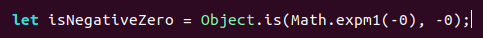
\includegraphics[width=300pt]{example1.png}
	\caption{Code which determines whether Math.expm1() returns 0 or -0}
  \label{fig:example1}
\end{figure}

The goal of the first stage of our exploit is to utilize the buggy fine-grained return type of
\texttt{Math.expm1()} to eliminate a bounds check which is in fact not safe, and allow us to access
memory outside the bounds of the array. The first step involves creating a variable which depends on
the result of our buggy function call. In other words, we need a way to distinguish between the
values 0 and -0. The only function useful to us in this case is \texttt{Object.is()}. In the code
segment shown in Figure \ref{fig:example1}, the variable \texttt{isNegativeZero} will be 1 if
\texttt{Math.expm1()} returns -0, and 0 otherwise. Running this line of code before it becomes 'hot'
and JIT optimzed will always store 1 into \texttt{isNegativeZero}, because the code is interpreted
directly and the native backing function for \texttt{Math.expm1()} returns -0. 

\begin{figure}
	\centering
	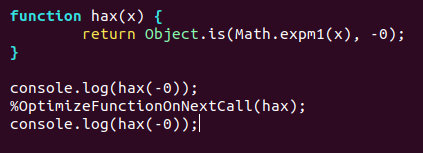
\includegraphics[width=300pt]{example2.png}
	\caption{The first call to hax() correctly prints 'true', but the second prints 'false' because the buggy JIT optimization folds the entire Object.is call to 'false'.}
  \label{fig:example2}
\end{figure}

This becomes interesting when we run the code after it has been JIT-optimized. Consider the code in
Figure \ref{fig:example2}. This code calls the function \texttt{hax} once without optimization, and
once with optimization. The \texttt{\%OptimizeFucntionOnNextCall} annotation is a macro which
can be invoked using the \texttt{--allow-natives-syntax} flag on the command line. These annotations
are only used for debugging, and in a real exploit this macro would be replaced with calling the
function a set number of times in a loop to achieve the level of optimization we want. Running this code prints \texttt{true} for the first call and \texttt{false}
for the second. Why? The first time the code runs, it is interpreted directly, and the engine
correctly evaluates -0 equal to -0. Before the second call, the JIT (incorrectly) optimizes the
function to native code, and in its analysis it incorrectly assumes \texttt{Math.expm1()} can never
return -0, since its return type is (erroneously) listed as a union of \texttt{PlainNumber} and
\texttt{NaN}. Therefore TurboFan assumes the \texttt{Object.is} call always evaluates to
\texttt{false}, and uses \textit{Folding} to reduce the variable \texttt{isNegativeZero} to the
constant \texttt{false}, thus breaking the semantics of the \texttt{Math.expm1()} function.

\subsection{Triggering an Out-of-Bounds Array Access}
\begin{figure}
	\centering
	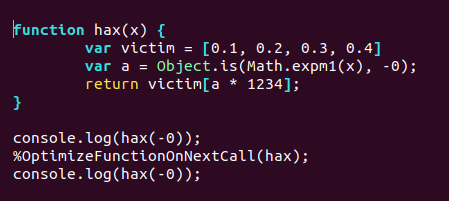
\includegraphics[width=300pt]{example3.png}
	\caption{First attempt at an out of bounds array access. This fails because the Object.is
	call folds to false, which prevents the out of bounds index.}
  \label{fig:example3}
\end{figure}
Now that we've triggered the bug, how can we turn it into a memory leak? The idea is to exploit the
bug to cause the JIT to remove an array bounds check in the optimized code, allowing us to read out
of bounds. Consider the code in Figure \ref{fig:example3} 
\section{Patch and Resolution}
\end{document}

